\setcounter{page}{1}

This thesis provides a general overview of the research that I have been developing since the beginning of my PhD studies in September, 2021. I could define myself as a curious, creative and open-minded person, following the so called \textit{IFISC attitude}, which means that I am always willing to learn new methods and address new problems, even though they are not directly related to my field of expertise. That is why, through this thesis many topics will be covered, from the study of human behavior and social systems, to the study of complex systems and network theory........

\section{\label{sec:scie_lands} Scientific Landscape}

This thesis adress the study of human behavior and social systems from a \textit{complex systems} perspective, which studies the emergence of collective phenomena that arise from the interactions of many individuals, and that cannot be understood by studying the behavior of individual agents in isolation (the so-called \textit{reductionist} approach) \cite{anderson1972more}. The study of collective phenomena has a long history in the natural sciences, specially in the branch of statistical physics \cite{stanley1971phase}. This branch traditionally studies the emergence of collective phenomena in physical systems, such as the phase transitions in magnetic materials via spin models \cite{onsager-1944}, the turbulence in fluids \cite{frisch1995turbulence}, the synchronization in oscillatory systems \cite{pikovsky2001universal}, or percolation \cite{stauffer-1985}. However, in recent years, the study of complex systems has evolved into the study of emergent phenomena beyond physical systems, such as biological \cite{prigogine1977self}, ecological \cite{may-2001}, economic \cite{arthur-1994}, and social systems \cite{castellano-2009}. Even though this branch of physics is relatively young, in 2021, the Nobel Prize in Physics was awarded to Syukuro Manabe, Klaus Hasselmann, and Giorgio Parisi for their contributions to the study of complex systems \cite{nobel-2021}, giving a recognition to this field in the scientific community \cite{bianconi2023complex}.

From the migration of birds \cite{roche-1997} to the spreading of a fake news through social media \cite{vosoughi-2018}, there are many examples of collective phenomena beyond the real of physics at which the study of complex systems can be applied. The cascade of failures in power grids \cite{dobson-2007}, the spread of a disease in a population \cite{anderson1991infectious}, the consensus in political elections \cite{anderson-2000}, the emergence of social norms \cite{ellickson-1999} are some examples of social collective behavior in which the global phenomena cannot be understood by looking at a single individual. Social and economic collective phenomena has been studied from a variety of perspectives (sociology, psychology, economics, political sciences...), which often relies on qualitative methods, such as interviews, surveys, or ethnographic studies \cite{bryman-2010}. However, the study of social systems from a complex systems perspective aims to provide a quantitative framework to understand the collective behavior, based on methodologies from statistical mechanics and network theory \cite{newman-book,barabasi-2013}. Nevertheless, this approach needs for a large amount of detailed data to validate theories and develop models, which historically has been a limitation for the study of social systems. It is in fact surprising how other branches of physics, where the typical scale of the phenomena is very large, as astrophysics, or very small, as particle physics, do not suffer from a lack of data, while the study of social systems, where the typical scale is human, has been historically limited by the lack of data.

Thankfully, the digital revolution has changed this picture, allowing the storage of large amounts of data generated by human activities, such as social media, mobile phones, or online platforms. Nowadays, every two year, more human socio-economic data is produced than during all the preceding years of human history together \cite{karsai2019computational}. This data, often referred to as \textit{Big data}, has opened a new era for the study of social systems at a large scale, together with a paradigm shift in the way we understand human behavior \cite{manyika-2011}. Nevertheless, this new era comes with an awareness, as the use of big data for the study of human behavior raises important ethical and privacy concerns, which need to be addressed in order to ensure the responsible use of data for the study of social systems \cite{boyd-2012}. Moreover, from the technical point of view, this huge amount of data needs for a set of computational and mathematical resources to be analyzed and modeled.From this demand, the field of \textit{Computational Social Science} has emerged, with the aim to develop new methods to study human behavior \cite{lazer-2009}. This branch of the complex systems science was born as a combination of methodologies borrowed from social sciences, such as sociology, psychology, or economics, with computational methods from computer science, such as machine learning, data mining, or network theory \cite{watts-2007}. This interdisciplinary approach has allowed to develop new methods for forecasting social phenomena and understanding the basic mechanism behind human interactions. 

One can differentiate two main approaches to build a representation of the reality from the data source. The first one is to focus on the prediction and forecasting of a certain social phenomena, such as the spread of a disease or the price of a stock. In this approach, the data is seen as a necessary input to our methodology to make quantitative predictions \cite{lazer-2009}. However, in this approach, the mechanisms behind the phenomena are often hidden in the data, and the model is seen as a black box that provides accurate predictions \cite{rudin-2019}. In this context, the use of machine learning \cite{murphy-2012} and deep learning \cite{goodfellow-2016} models are  very popular, as they are able to capture complex patterns in the data. The second approach is to focus on the understanding of the mechanisms behind the phenomena. In this approach, the data is seen as a problem to be understood, an observation from which we can extract qualitative behaviors and patterns \cite{axelrod-1997}. In this context, the aim is to develop very simple models that are able to reproduce the main features of the data, and to extract the basic mechanisms behind the phenomena.

Following the later approach, network science has a critical role in the study of socio-economic systems, as it provides a natural framework to study the interactions between individuals. A network, or graph, is a mathematical representation of a set of nodes (individuals) connected by links (interactions), which allows to study the structure of the interactions and the dynamics of the system. The study of networks has a long history in the natural sciences, from the neurons network in the brain \cite{sporns-2004} to food webs in an ecosystem \cite{ings-2008, elith-2009, bastolla-2009}. However, in recent years, new data sources lead to the discovery that complex properties and heterogeneities, present in most social systems, need for a topological description in terms of a complex network \cite{newman-book, dorogovtsev2002evolution, kilduff2003social}. A complex network can be defined is a network that exhibits non-trivial topological properties, which we will explain later on this thesis. These properties are often found in social networks, such as a social media \cite{dunbar-2015}, the collaboration network of scientists \cite{newman-coll-2001,radicchi-2008}, or international conflicts \cite{hafnerburton-2009, diaz2023network}. In particular, the study of information spreading as a dynamical system on networks has allowed to understand how information spreads through a social system and how consensus emerges.

Contagion of information has been a topic of interest for many social scientists. Early theoretical frameworks,influenced by psychological and sociological theories, show how individuals in a crowd lose their sense of self and are more susceptible to the ideas and emotions of the crowd \cite{le2023crowd}. Social imitation of behaviors and ideas was proposed as a mechanism for social change, facilitated by close contact and communication among individuals \cite{kanter-1971}. Similarly, peer pressure was also proposed another possible mechanism, where individuals are influenced by their peers to adopt certain behaviors or ideas \cite{granovetter-1978, brown-1986}. However, until now these theoretical dissertations were not supported by quantitative results with real data analysis. For example, the spread of innovations \cite{rogers2014}, the diffusion of information \cite{valente-1996}, or the spread of diseases \cite{anderson1991infectious} are some examples of social phenomena where we can test if the traditional theoretical frameworks are able to reproduce the data.

Beyond the network structure and the contagion dynamics, there is a third ingredient that is critical for the study of social systems: the human temporal interactions. Human interactions exhibit complex activity patterns that are difficult to understand and to model, since there are a lot of mechanisms that drive the human behavior. For example, the human activity patterns can be driven by the circadian rhythms \cite{roenneberg-2013}, bursty interactions \cite{Barabasi2005Bursts}, cascades \cite{watts-2002}, periodic commuting behaviors \cite{gonzalez2008understanding}, recurring patterns in online behavior \cite{Lazer2009CompSocSci}, etc. All this effects are embedded to the socio-economic environment and the social network structure, so they cannot be ignored. In fact, there are studies that show how the temporal patterns of human interactions can affect the spreading of information \cite{Holme2012Temporal}, changing the nature of the dynamic process dramatically \cite{karsai-2011}.

In this thesis, we use the complex systems approach to try to understand the consequences of the irregular human activity patterns (temporal interactions) in many socio-economic models. Under this perspective, we will apply tools borrowed from computational social science and network theory to study the problems under this umbrella, such as the spread of information, the consensus emergence, etc, problems associated traditionally to other research areas, which are really important to understand.

\section{\label{sec:Challenges of Computational Social Science} Challenges of Computational Social Science}

Since the research in this field is relatively new, the methodology is not yet well stablish, but it follows the traditional approach from natural sciences, like physics, but with new relevant techniques adapted to the specific problem to address. In this section, we introduce some of the challenges the study of human behavior faces, and which are the computational methods that are used to explore a solution.

Regarding to the data availability, digital behavioral data provides a detailed look at human activities in their usual environments, capturing information about where, when, and how people behave \cite{Eagle2006RealityMining}. This type of data is great because it avoids the common biases seen in older research methods and gives us a clearer picture across a large number of people \cite{lazer-2009,chen-2014}. Instead of relying on limited lab studies or broad census data, the data is now collected from real-world interactions, which is stored from digital devices and platforms that people use in their daily lives \cite{Eckmann2004Entropy,blondel-2015,artime-2017}. However, this data is like a picture of a black hole, neither you cannot observe it in a controlled environment nor analyzing the response to a stimuli \cite{lazer-2014}. Also, not everyone is equally represented in digital data, especially in poor countries, where the use of technology is less popularized \cite{zook-2017}. Ethically, there are also big concerns about collecting and using personal data without people knowing it \cite{boyd-2012, de-montjoye-2013}, which has pushed for stricter laws to protect privacy and ensure people have control over their own data.

Regarding to data analysis, several statistical methodologies have been designed to manage small data sets in social and economic research, giving rise to meaningful models and techniques \cite{stevens-2012, gelman-2006}. These traditional techniques have evolved to accommodate the large data volumes seen in modern statistical analysis \cite{hastie-2013}, where the challenge is no longer sample size but the data heterogeneity. Using tools such as data mining, statistical tests, etc, we can extract patterns and convert large noisy data sets into intelligible knowledge \cite{witten-2005}. Furthermore, network analysis is helpful to analyze several datasets from a different perspective, highlighting the crossed interactions between the different variables \cite{newman-book, clauset-2008}. The use of null models \cite{perry2012null,gauvin-2022} is an example of a common practice in network analysis, in which the interactions are rewired (reshuffled), breaking the correlations, to compare if the macroscopic properties of the network are meaningful or not.

Regarding to understand and model human behavior through three main approaches. Statistical Models are used to identify correlations and make individualized predictions but mainly generate hypotheses without exploring underlying mechanisms, for example, machine learning \cite{murphy-2012}, bayesian inference \cite{gelman1995bayesian}, deep learning \cite{goodfellow-2016}, etc. Mechanistic Models, inspired by physics, simulate emergent behaviors from simpler entity interactions, offering robust scenario testing but often simplifying individual differences \cite{axelrod2006agent}. Agent-based modeling (ABM) emerged as a particularly influential mechanistic approach, enabling scientists to create and study systems of interacting agents (individuals or collective entities) and observe emergent behaviors from simple rules of interaction \cite{epstein1999agent}.On the other hand, data-driven models blend real-world data with synthetic frameworks to focus on specific mechanisms, allowing for realistic simulations and in-depth analysis of the dynamics. The availability to address problems from these 3 perspectives is crucial in the branch of computational social science, and enhances understanding by forming, testing, and refining hypotheses \cite{watts2004new}.

Finally, the scope of applications in computational social science goes beyond the study of social systems. Generative and data-driven modeling are employed in diverse scenarios such as managing crowd dynamics, improving cooperative behaviors, optimizing traffic and public transport systems, facilitating product and service adoption, and forecasting global pandemics. This multifaceted field is becoming increasingly relevant in modern techno-social societies \cite{vespignani2009predicting}, enhancing the quantitative nature of social sciences and leading the shift towards a digital, data-driven paradigm across science, technology, and various applied domains. One example of these applications, related to contagion dynamics, are the fake news observatories \cite{Polis-observatory, EDMO-observatory, committed-observatory-2023}, which are platforms that monitor the spread of fake news in social media, and provide tools to detect and give feedback to the users.

\section{\label{sec:Terminology and general concepts} Terminology and general concepts}

In this section, we briefly introduce general definitions and concepts, which will be used through the thesis. We introduce basic concepts of complex networks, and some tools that are used to model social and economic systems. Furthermore, we briefly describe models that are used, via complex networks, to study human behavior and social systems in general.

\subsection{\label{subsec:Complex networks} Complex networks}

\begin{figure}
    \centering
    \captionsetup{font=sf}
    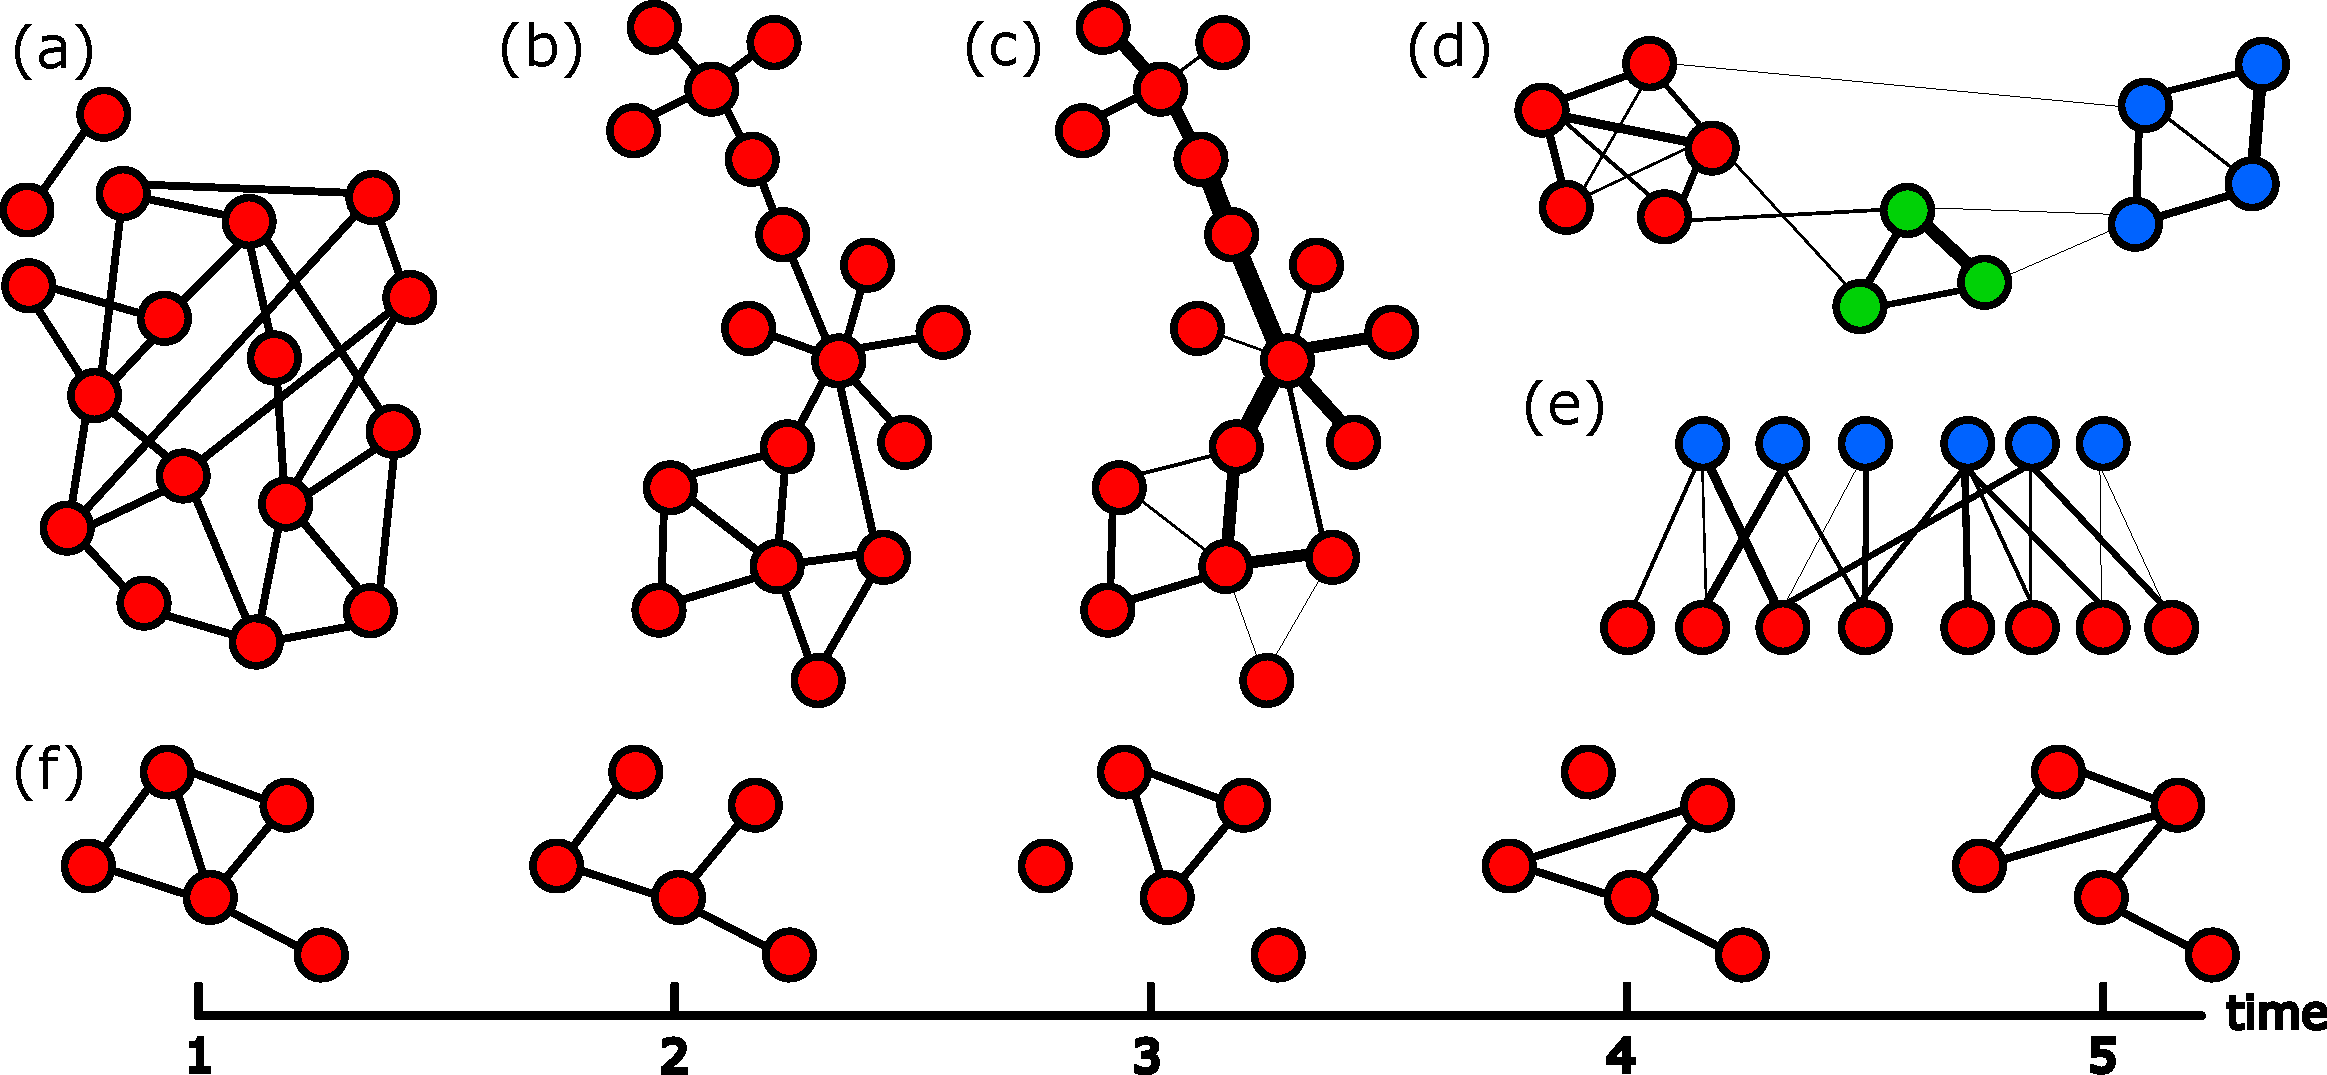
\includegraphics[width=\textwidth]{Figs/Introduction/network_plot.pdf}
    \caption[Different network types]{.}
    \label{fig:netwotk_types}
\end{figure}

A network is a mathematical representation of a set of nodes connected by links. This simple definition allows to map the architecture of many complex systems by identifying the interactions between the different elements. This topology allows us to quantify how close or far two nodes are (path length), how many central a node is (degree), how many triangles are formed by the neighbors of a node (clustering), etc. As I understood it through this years, what makes a network complex is having a short path length, such that average distance between two nodes is relatively small, high levels of clustering, such that nodes tend to form triangles, and a degree distribution with a fat tail, such that there are a few nodes with a very high degree. These properties are often found in many social, biological and economic complex systems, such as social media, ecological networks, or financial systems.

To create synthetic networks with the same properties to complex networks, we use stochastic models that, from few nodes, describe how we need to grow the network to reach our goal \cite{posfai2016network}. One popular example is the Erd\H{o}s-Renyi model \cite{erdos1960evolution}, which grows the network by adding links between nodes with a certain probability $p$. This model is useful to study the emergence of the giant component in a network, which is the largest connected component in the network. However, this model has a binomial degree distribution, and the path length is too large to reproduce a real complex network. Another popular example is the Watts-Strogatz model \cite{watts1998collective}, which grows the network by adding links between nodes with a certain probability $p$, and then rewiring the links with a certain probability $q$. This model is useful to study the emergence of small-world networks, which have a short path length and a high clustering. However, the degree distribution is still binomial, which is not useful to study the emergence of hubs in a network \cite{newman2003structure}. Finally, the Barab\'asi-Albert model \cite{barabasi1999emergence} grows the network by adding nodes that attach to the present nodes with a probability proportional to the degree of the nodes. This process is called \textit{preferential attachment}, and it is useful to reproduce the fat tail degree distribution or, in other words, the emergence of hubs (nodes with a very high degree) in a network. If instead of adding nodes according to a certain rule, we want to directly impose a certain observed degree distribution, we can use the configuration model \cite{newman-book}, which is a generalization of the Erd\H{o}s-R\'enyi model in which we start from a set of nodes disconnected, each one with a certain number of stubs, and then we connect the stubs with a certain probability. It can be shown that the clustering in networks generated using the configuration model for any degree distribution is proportional to $1/N$, where $N$ is the number of nodes in the network. This means that for large networks, the clustering is very small, a feature that we will se its useful to describe agent based models in networks.

Until now, we considered only simple networks, in which the links are binary (there is link or there is not). However, we can consider that links are weighted, which means that each link has a certain number (or another quality) associated to it \cite{barrat2004architecture}. This representation is useful to describe the strength of the interactions between nodes. For example, the railway network is a simple network that connects railway stations via the railway lines, but the weight of each line is the number of trains or the number of passengers that travel through it \cite{latora-2002}. This representation is very usefull when we have a system very densely connected, but there are some links that have a higher importance or are more saturated than others, depending on the context. Also, this representation allows us to map any correlation matrix as a weighted network, which might be useful to identify the more correlated and anticorrelated elements in a system \cite{onnela-2003,tumminello-2005}.

In fact, a common trait that is found in complex systems is the presence of communities, which are groups of nodes that are more connected between them than with the rest of the network \cite{girvan-2002}. For example, communities can represent groups of friends, families, or work colleagues, which are more likely to share information and to interact between them \cite{newman2001structure}. To identify communities in a network, we can use community detection algorithms, which are algorithms that group nodes in the network in a way that maximizes the number of links inside the groups and minimizes the number of links between the groups \cite{lancichinetti-2008,fortunato2010community}. One popular example is the Louvain algorithm \cite{blondel-2008}, which is a greedy algorithm that optimizes a modularity function, which is a measure of the quality of the partition of the network. Another popular example is the Infomap algorithm \cite{rosvall-2008}, which is a flow-based algorithm that optimizes a map equation, which is a measure of the quality of the partition of the network. These algorithms are useful to identify the structure of the network, and to understand the dynamics of the system.

On the other hand, there are networks in which by definition there are two groups, and there are just links between the two groups (not between elements in the same group). These networks are called bipartite networks \cite{newman2001structure}, and they are useful to represent systems in which there are two types of elements, and there are interactions between the two types of elements \cite{latapy-2008}. For example, online platforms to see movies and tv shows, such as Netflix \cite{netflix} and HBO \cite{HBO}, can be considered as bipartite network in which there are users and movies, and there are links between users and movies if the user has watched the movie. This representation is useful to study the recommendation systems, which are systems that recommend items to users based on their preferences \cite{ricci-2011}. Moreover, bipartite networks allows us to project into a weighted network of nodes of the same type, where the weight of the link is typically computed and normalized by the number of common neighbors (of the other type) between the two nodes \cite{newman-2001-collaboration}. In the case of the movie recommendation system, we can project the bipartite network into a weighted network of users, where the weight of the link between two users is the number of movies that they have watched in common. The projection is useful to study the social interactions between users, and to identify communities in the network.

Finally, there are networks in which the interactions between nodes are not static, but they evolve in time (temporal networks) \cite{Holme2012Temporal}. These networks are useful to represent systems in which the interactions between nodes change in time \cite{Perra2012ActivityDriven}. For example, the phone calls in a group of friends is a temporal network, in which the links are the phone calls that take place at a certain time window. This representation is useful to study the dynamics of the system, and to understand how the interactions between nodes change in time \cite{karsai-2011} or if they exhibit periodic patterns \cite{Jo2012Circadian}.

\subsection{\label{subsec:Agent-based models} Agent-based models}

Agent-based models are a class of computational models for simulating the actions and interactions of autonomous agents (both individual or collective entities) with a view to assessing their effects on the system as a whole. They are used to understand the collective behavior of the agents, and the emergent properties of the system. The agents can be individuals, groups, or organizations, and if the network topology is necessary, the agents are placed in the nodes of a network. The agents are characterized its state, which may be discrete or continuous, and its behavior or update rules. The rules, deterministic or stochastic, are the recipe that the agents need to follow to interact with its environment. For example, for the Voter model, an agent has an state that represents one of the two opinions and the update rules are just to imitate the state of a neighbor.

An important ingredient when we perform agent-based simulations is the order in which nodes are updated. The order can be synchronous, in which all nodes are updated at the same time, or asynchronous, in which nodes are updated one by one. Nevertheless, the synchronous update may lead to problematic schemes, in which the system may get stuck in a periodic or chaotic solution. Performing simulations in asyncronous order, the order can also be random, in which nodes are updated one by one in a random order, or sequential, in which nodes are updated in a certain order. A common order is to just follow a random asynchronous update (RAU), which avoids biases and allows to explore the space of solutions in a more efficient way. Nevertheless, the sequential asynchronous update (SAU) is useful in cases reduce the computational cost, as the system may converge faster to a solution. 

Usually, in agent based-models, these simulation steps are repeated until a stationary state is reached (if exists). To do so, one can perform Monte Carlo simulations, which are a class of computational algorithms that rely on repeated random sampling to obtain numerical results. In these simulations, a time step (Monte Carlo step) is defined as the time in which, on average, each node is updated once. These are useful to explore the space of solutions, and to understand the dynamics of the system. A different approach is to use the Gillespie algorithm, which is a stochastic simulation algorithm that generates a trajectory of the system by sampling the time of the next event and the event that will take place. This algorithm is useful because, since the time is not fixed, we avoid time steps in which nothing happens, and we can explore the dynamics of the system in a more efficient way.

Finally, the output of this simulations is a set of relevant statistics that describe the system's trajectory or the stationary state. These statistics can be the average opinion of the agents, the number of clusters in the network, the number of links between clusters, the average interface density, etc. An ensemble of simulations is ofter performed to explore the space of possible trajectories and solutions, and to understand the robustness of the results. This ensemble can be performed by simply repeating the stochastic simulation, or by changing a trait of the system, such as the initial conditions of the system, or the realization of the network.

\section{\label{sec:Datasets} Datasets}

\begin{figure}
    \centering
    \captionsetup{font=sf}
    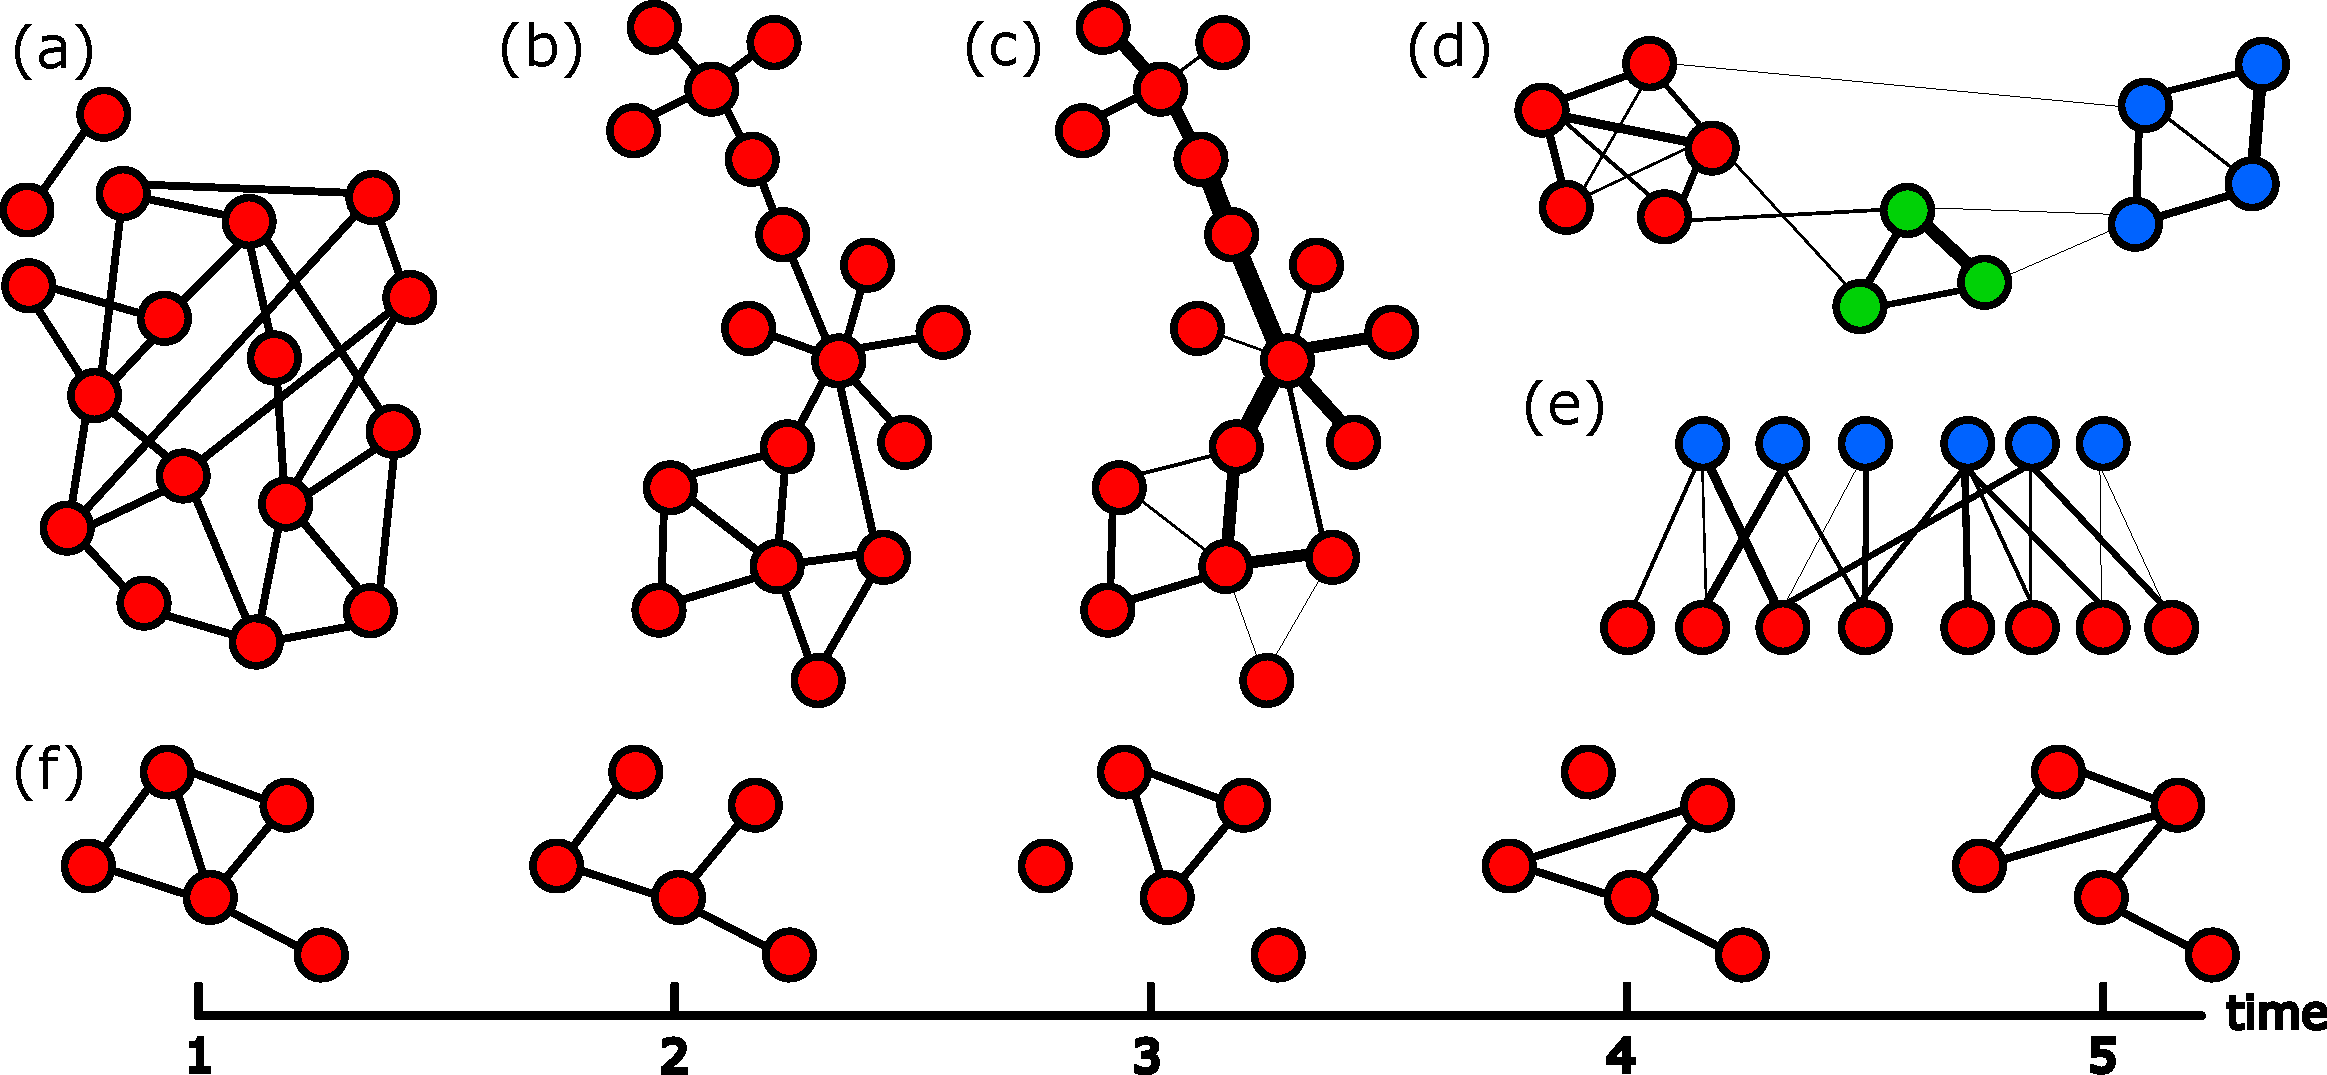
\includegraphics[width=\textwidth]{Figs/Introduction/network_plot.pdf}
    \caption[Amount of adds per cell]{.}
    \label{fig:netwotk_types}
\end{figure}

- We used the idealista dataset

- The strong point of the idealista dataset is that it contains information about the real estate market in Spain, and that it is a large dataset that contains information about the real estate market in Spain.

- The missing point of the idealista dataset is that it contains information about the real estate market in Spain, and that it is a large dataset that contains information about the real estate market in Spain.
